\documentclass[class=article,border=5pt,tikz]{standalone}
\usetikzlibrary{intersections,angles,quotes}

\begin{document}

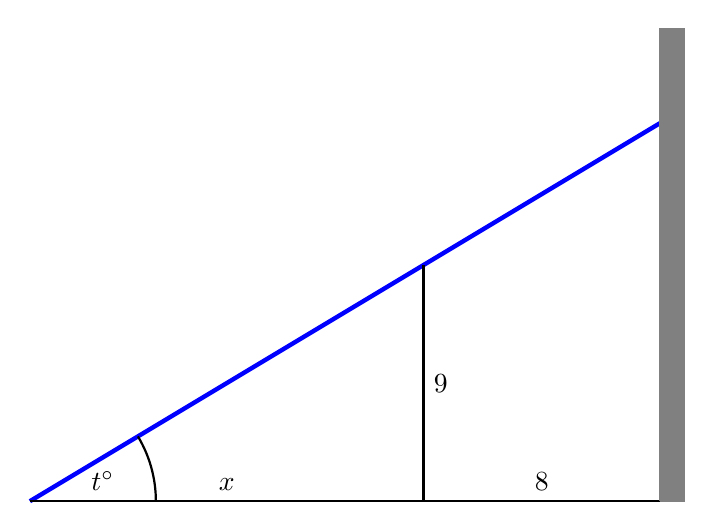
\begin{tikzpicture}[thick,x=1cm,y=1cm]
\coordinate (A) at (0,0);
\coordinate (B) at (5,0);
\coordinate (C) at (8,0);
\coordinate (D) at (5,3);
\coordinate (E) at (8,4.8);
\coordinate (F) at (8,6);
\coordinate (G) at (8.3,6);
\coordinate (H) at (8.3,0);
\draw [ultra thick, blue] (A) -- (E); 
\draw (B) -- (D) node[midway, right]{$9$};
\draw (A) -- (B) node[midway,above]{$x$} -- (C) node[midway,above]{$8$};
\draw [gray,fill=gray] (C) -- (F) -- (G) -- (H) -- (C);
\draw pic ["$t^{\circ}$",draw,thick,angle radius=1.6cm] {angle = C--A--E};
\end{tikzpicture}

\end{document}

